\section{Данные, усреднённые по 0.5 с}

\subsection{Зависимость скорости колеса от тока двигателя}

\subsubsection{Гладкая поверхность}

\begin{figure}[H]
    \centering
    \includegraphics[width=\textwidth]{for_research_movement_direction/wheel_velocity_vs_motor_current/averaged_data/separate_with_set_velocity/table/motor1.pdf}
    \caption{Зависимость скорости колеса от тока 1-го двигателя на гладкой поверхности}
\end{figure}

\begin{figure}[H]
    \centering
    \includegraphics[width=\textwidth]{for_research_movement_direction/wheel_velocity_vs_motor_current/averaged_data/separate_with_set_velocity/table/motor2.pdf}
    \caption{Зависимость скорости колеса от тока 2-го двигателя на гладкой поверхности}
\end{figure}

\begin{figure}[H]
    \centering
    \includegraphics[width=\textwidth]{for_research_movement_direction/wheel_velocity_vs_motor_current/averaged_data/separate_with_set_velocity/table/motor3.pdf}
    \caption{Зависимость скорости колеса от тока 3-го двигателя на гладкой поверхности}
\end{figure}

\subsubsection{Серая поверхность}

\begin{figure}[H]
    \centering
    \includegraphics[width=\textwidth]{for_research_movement_direction/wheel_velocity_vs_motor_current/averaged_data/separate_with_set_velocity/gray/motor1.pdf}
    \caption{Зависимость скорости колеса от тока 1-го двигателя на серой поверхности}
\end{figure}

\begin{figure}[H]
    \centering
    \includegraphics[width=\textwidth]{for_research_movement_direction/wheel_velocity_vs_motor_current/averaged_data/separate_with_set_velocity/gray/motor2.pdf}
    \caption{Зависимость скорости колеса от тока 2-го двигателя на серой поверхности}
\end{figure}

\begin{figure}[H]
    \centering
    \includegraphics[width=\textwidth]{for_research_movement_direction/wheel_velocity_vs_motor_current/averaged_data/separate_with_set_velocity/gray/motor3.pdf}
    \caption{Зависимость скорости колеса от тока 3-го двигателя на серой поверхности}
\end{figure}

\subsubsection{Зелёная поверхность}

\begin{figure}[H]
    \centering
    \includegraphics[width=\textwidth]{for_research_movement_direction/wheel_velocity_vs_motor_current/averaged_data/separate_with_set_velocity/green/motor1.pdf}
    \caption{Зависимость скорости колеса от тока 1-го двигателя на зелёной поверхности}
\end{figure}

\begin{figure}[H]
    \centering
    \includegraphics[width=\textwidth]{for_research_movement_direction/wheel_velocity_vs_motor_current/averaged_data/separate_with_set_velocity/green/motor2.pdf}
    \caption{Зависимость скорости колеса от тока 2-го двигателя на зелёной поверхности}
\end{figure}

\begin{figure}[H]
    \centering
    \includegraphics[width=\textwidth]{for_research_movement_direction/wheel_velocity_vs_motor_current/averaged_data/separate_with_set_velocity/green/motor3.pdf}
    \caption{Зависимость скорости колеса от тока 3-го двигателя на зелёной поверхности}
\end{figure}

\subsubsection{Сравнение распределение данных по поверхностям}

\begin{figure}[H]
    \centering
    \begin{subfigure}{0.45\textwidth}
        \centering
        \includegraphics[width=\textwidth]{for_research_movement_direction/wheel_velocity_vs_motor_current/averaged_data/separate_with_surface_type/motor1.pdf}
        \caption{двигатель 1}
    \end{subfigure}
    \hspace{0.005\textwidth}
    \begin{subfigure}{0.45\textwidth}
        \centering
        \includegraphics[width=\textwidth]{for_research_movement_direction/wheel_velocity_vs_motor_current/averaged_data/separate_with_surface_type/motor3.pdf}
        \caption{двигатель 3}
    \end{subfigure} \\
    \vspace{4pt}
    \centering
    \begin{subfigure}{0.45\textwidth}
        \centering
        \includegraphics[width=\textwidth]{for_research_movement_direction/wheel_velocity_vs_motor_current/averaged_data/separate_with_surface_type/motor2.pdf}
        \caption{двигатель 2}
    \end{subfigure}
    \caption{Зависимость скорости колеса от тока двигателя}
\end{figure}

Фактически, было получено семейство электромеханических характеристик двигателей робота при разных напряжениях якоря или разных задающих скоростях (на рисунке \ref{fig:electromechanic_characteristics} зелёным цветом).

\begin{figure}[H]
    \centering
    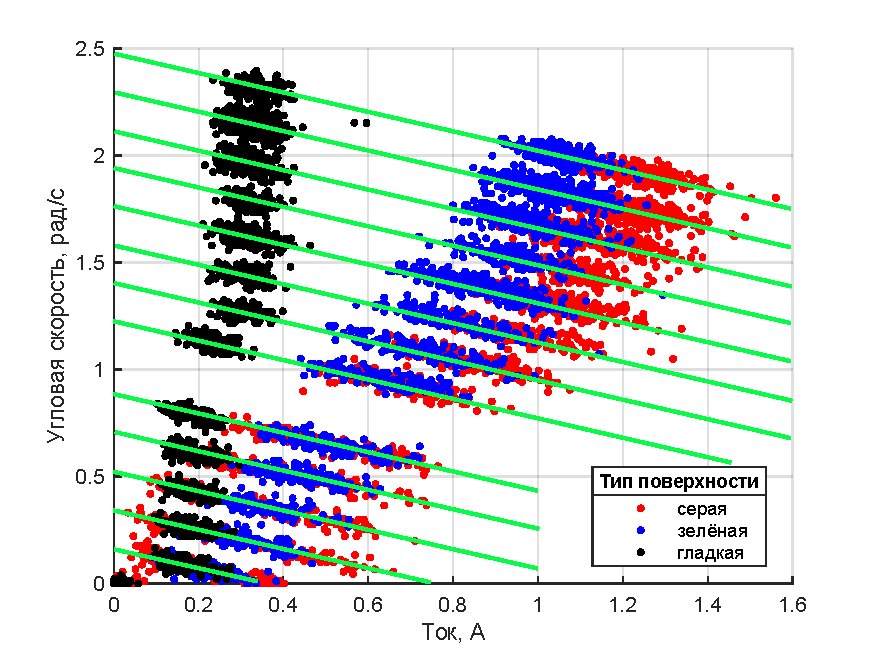
\includegraphics[width=0.6\textwidth]{motor1 electromechanic characteristics.pdf}
    \caption{Примерный вид семейства электромеханических характеристик для 1-го двигателя}
    \label{fig:electromechanic_characteristics}
\end{figure}

\subsection{Зависимость тока от направления движения робота}

\begin{figure}[H]
    \centering
    \begin{subfigure}{0.45\textwidth}
        \centering
        \includegraphics[width=\textwidth]{for_research_movement_direction/polar_current/half_second_averaging/table/motor1.pdf}
        \caption{двигатель 1}
    \end{subfigure}
    \hspace{0.005\textwidth}
    \begin{subfigure}{0.45\textwidth}
        \centering
        \includegraphics[width=\textwidth]{for_research_movement_direction/polar_current/half_second_averaging/table/motor3.pdf}
        \caption{двигатель 3}
    \end{subfigure} \\
    \vspace{4pt}
    \centering
    \begin{subfigure}{0.45\textwidth}
        \centering
        \includegraphics[width=\textwidth]{for_research_movement_direction/polar_current/half_second_averaging/table/motor2.pdf}
        \caption{двигатель 2}
    \end{subfigure}
    \caption{Зависимость тока двигателя от направления движения робота на гладкой поверхности}
\end{figure}

\begin{figure}[H]
    \centering
    \begin{subfigure}{0.49\textwidth}
        \centering
        \includegraphics[width=\textwidth]{for_research_movement_direction/polar_current/half_second_averaging/gray/motor1.pdf}
        \caption{двигатель 1}
    \end{subfigure}
    \hspace{0.005\textwidth}
    \begin{subfigure}{0.49\textwidth}
        \centering
        \includegraphics[width=\textwidth]{for_research_movement_direction/polar_current/half_second_averaging/gray/motor3.pdf}
        \caption{двигатель 3}
    \end{subfigure} \\
    \vspace{4pt}
    \centering
    \begin{subfigure}{0.49\textwidth}
        \centering
        \includegraphics[width=\textwidth]{for_research_movement_direction/polar_current/half_second_averaging/gray/motor2.pdf}
        \caption{двигатель 2}
    \end{subfigure}
    \caption{Зависимость тока двигателя от направления движения робота на серой поверхности}
\end{figure}

\begin{figure}[H]
    \centering
    \begin{subfigure}{0.49\textwidth}
        \centering
        \includegraphics[width=\textwidth]{for_research_movement_direction/polar_current/half_second_averaging/green/motor1.pdf}
        \caption{двигатель 1}
    \end{subfigure}
    \hspace{0.005\textwidth}
    \begin{subfigure}{0.49\textwidth}
        \centering
        \includegraphics[width=\textwidth]{for_research_movement_direction/polar_current/half_second_averaging/green/motor3.pdf}
        \caption{двигатель 3}
    \end{subfigure} \\
    \vspace{4pt}
    \centering
    \begin{subfigure}{0.49\textwidth}
        \centering
        \includegraphics[width=\textwidth]{for_research_movement_direction/polar_current/half_second_averaging/green/motor2.pdf}
        \caption{двигатель 2}
    \end{subfigure}
    \caption{Зависимость тока двигателя от направления движения робота на зелёной поверхности}
\end{figure}

\begin{figure}[H]
    \centering
    \begin{subfigure}{0.49\textwidth}
        \centering
        \includegraphics[width=\textwidth]{for_research_movement_direction/polar_current/half_second_averaging/motor1.pdf}
        \caption{двигатель 1}
    \end{subfigure}
    \hspace{0.005\textwidth}
    \begin{subfigure}{0.49\textwidth}
        \centering
        \includegraphics[width=\textwidth]{for_research_movement_direction/polar_current/half_second_averaging/motor3.pdf}
        \caption{двигатель 3}
    \end{subfigure} \\
    \vspace{4pt}
    \centering
    \begin{subfigure}{0.49\textwidth}
        \centering
        \includegraphics[width=\textwidth]{for_research_movement_direction/polar_current/half_second_averaging/motor2.pdf}
        \caption{двигатель 2}
    \end{subfigure}
    \caption{Сравнение зависимостей тока двигателя от направления движения робота на разных типах поверхности}
\end{figure}

\subsubsection{Зависимость уголовой скорости колеса от направления движения робота}

\begin{figure}[H]
    \centering
    \begin{subfigure}{0.45\textwidth}
        \centering
        \includegraphics[width=\textwidth]{for_research_movement_direction/polar_velocity/half_second_averaging/table/wheel1.pdf}
        \caption{колесо 1}
    \end{subfigure}
    \hspace{0.005\textwidth}
    \begin{subfigure}{0.45\textwidth}
        \centering
        \includegraphics[width=\textwidth]{for_research_movement_direction/polar_velocity/half_second_averaging/table/wheel3.pdf}
        \caption{колесо 3}
    \end{subfigure} \\
    \vspace{4pt}
    \centering
    \begin{subfigure}{0.45\textwidth}
        \centering
        \includegraphics[width=\textwidth]{for_research_movement_direction/polar_velocity/half_second_averaging/table/wheel2.pdf}
        \caption{колесо 2}
    \end{subfigure}
    \caption{Зависимость уголовой скорости колеса от направления движения робота на гладкой поверхности}
\end{figure}

\begin{figure}[H]
    \centering
    \begin{subfigure}{0.49\textwidth}
        \centering
        \includegraphics[width=\textwidth]{for_research_movement_direction/polar_velocity/half_second_averaging/gray/wheel1.pdf}
        \caption{колесо 1}
    \end{subfigure}
    \hspace{0.005\textwidth}
    \begin{subfigure}{0.49\textwidth}
        \centering
        \includegraphics[width=\textwidth]{for_research_movement_direction/polar_velocity/half_second_averaging/gray/wheel3.pdf}
        \caption{колесо 3}
    \end{subfigure} \\
    \vspace{4pt}
    \centering
    \begin{subfigure}{0.49\textwidth}
        \centering
        \includegraphics[width=\textwidth]{for_research_movement_direction/polar_velocity/half_second_averaging/gray/wheel2.pdf}
        \caption{колесо 2}
    \end{subfigure}
    \caption{Зависимость уголовой скорости колеса от направления движения робота на серой поверхности}
\end{figure}

\begin{figure}[H]
    \centering
    \begin{subfigure}{0.49\textwidth}
        \centering
        \includegraphics[width=\textwidth]{for_research_movement_direction/polar_velocity/half_second_averaging/green/wheel1.pdf}
        \caption{колесо 1}
    \end{subfigure}
    \hspace{0.005\textwidth}
    \begin{subfigure}{0.49\textwidth}
        \centering
        \includegraphics[width=\textwidth]{for_research_movement_direction/polar_velocity/half_second_averaging/green/wheel3.pdf}
        \caption{колесо 3}
    \end{subfigure} \\
    \vspace{4pt}
    \centering
    \begin{subfigure}{0.49\textwidth}
        \centering
        \includegraphics[width=\textwidth]{for_research_movement_direction/polar_velocity/half_second_averaging/green/wheel2.pdf}
        \caption{колесо 2}
    \end{subfigure}
    \caption{Зависимость уголовой скорости колеса от направления движения робота на зелёной поверхности}
\end{figure}

Из графиков видно, что ток и угловая скорость имеет похожую зависимость от направления движения робота. При этом, зависимость угловой скорость напрямую обусловлено кинематикой мобильной платформы. А ток в свою очередь зависит уже от задающей скорости/напряжения или выходной скорости. Проверим это.

\subsubsection{Корреляция между угловой скоростью и током двигателя}

\begin{figure}[H]
    \centering
    \begin{subfigure}{0.49\textwidth}
        \centering
        \includegraphics[width=\textwidth]{for_research_movement_direction/correlation_between_motor_current_and_wheel_velocity/table/motor1.pdf}
        \caption{двигатель 1}
    \end{subfigure}
    \hspace{0.005\textwidth}
    \begin{subfigure}{0.49\textwidth}
        \centering
        \includegraphics[width=\textwidth]{for_research_movement_direction/correlation_between_motor_current_and_wheel_velocity/table/motor3.pdf}
        \caption{двигатель 3}
    \end{subfigure} \\
    \vspace{4pt}
    \centering
    \begin{subfigure}{0.49\textwidth}
        \centering
        \includegraphics[width=\textwidth]{for_research_movement_direction/correlation_between_motor_current_and_wheel_velocity/table/motor2.pdf}
        \caption{двигатель 2}
    \end{subfigure}
    \caption{Матрица корреляции между уголовой скоростью и током двигателя на гладкой поверхности}
\end{figure}

\begin{figure}[H]
    \centering
    \begin{subfigure}{0.49\textwidth}
        \centering
        \includegraphics[width=\textwidth]{for_research_movement_direction/correlation_between_motor_current_and_wheel_velocity/gray/motor1.pdf}
        \caption{двигатель 1}
    \end{subfigure}
    \hspace{0.005\textwidth}
    \begin{subfigure}{0.49\textwidth}
        \centering
        \includegraphics[width=\textwidth]{for_research_movement_direction/correlation_between_motor_current_and_wheel_velocity/gray/motor3.pdf}
        \caption{двигатель 3}
    \end{subfigure} \\
    \vspace{4pt}
    \centering
    \begin{subfigure}{0.49\textwidth}
        \centering
        \includegraphics[width=\textwidth]{for_research_movement_direction/correlation_between_motor_current_and_wheel_velocity/gray/motor2.pdf}
        \caption{двигатель 2}
    \end{subfigure}
    \caption{Матрица корреляции между уголовой скоростью и током двигателя на серой поверхности}
\end{figure}

\begin{figure}[H]
    \centering
    \begin{subfigure}{0.49\textwidth}
        \centering
        \includegraphics[width=\textwidth]{for_research_movement_direction/correlation_between_motor_current_and_wheel_velocity/green/motor1.pdf}
        \caption{двигатель 1}
    \end{subfigure}
    \hspace{0.005\textwidth}
    \begin{subfigure}{0.49\textwidth}
        \centering
        \includegraphics[width=\textwidth]{for_research_movement_direction/correlation_between_motor_current_and_wheel_velocity/green/motor3.pdf}
        \caption{двигатель 3}
    \end{subfigure} \\
    \vspace{4pt}
    \centering
    \begin{subfigure}{0.49\textwidth}
        \centering
        \includegraphics[width=\textwidth]{for_research_movement_direction/correlation_between_motor_current_and_wheel_velocity/green/motor2.pdf}
        \caption{двигатель 2}
    \end{subfigure}
    \caption{Матрица корреляции между уголовой скоростью и током двигателя на зелёной поверхности}
\end{figure}

\subsection{Сравнение формы полярных кривых среднего значения тока на каждом направлении}

\begin{figure}[H]
    \centering
    \begin{subfigure}{0.49\textwidth}
        \centering
        \includegraphics[width=\textwidth]{for_research_movement_direction/polar_current/full_averaging/motor1.pdf}
        \caption{двигатель 1}
    \end{subfigure}
    \hspace{0.005\textwidth}
    \begin{subfigure}{0.49\textwidth}
        \centering
        \includegraphics[width=\textwidth]{for_research_movement_direction/polar_current/full_averaging/motor3.pdf}
        \caption{двигатель 3}
    \end{subfigure} \\
    \vspace{4pt}
    \centering
    \begin{subfigure}{0.49\textwidth}
        \centering
        \includegraphics[width=\textwidth]{for_research_movement_direction/polar_current/full_averaging/motor2.pdf}
        \caption{двигатель 2}
    \end{subfigure}
    \caption{Зависимость среднего значения тока от направления движения робота}
\end{figure}

\subsection{Зависимость проскальзывания от направления движения}

\begin{figure}[H]
    \centering
    \begin{subfigure}{0.49\textwidth}
        \centering
        \includegraphics[width=\textwidth]{for_research_movement_direction/polar_slippage/half_second_averaging/table/motor1.pdf}
        \caption{двигатель 1}
    \end{subfigure}
    \hspace{0.005\textwidth}
    \begin{subfigure}{0.49\textwidth}
        \centering
        \includegraphics[width=\textwidth]{for_research_movement_direction/polar_slippage/half_second_averaging/table/motor3.pdf}
        \caption{двигатель 3}
    \end{subfigure} \\
    \vspace{4pt}
    \centering
    \begin{subfigure}{0.49\textwidth}
        \centering
        \includegraphics[width=\textwidth]{for_research_movement_direction/polar_slippage/half_second_averaging/table/motor2.pdf}
        \caption{двигатель 2}
    \end{subfigure}
    \caption{Зависимость проскальзывания от направления движения робота на гладкой поверхности}
\end{figure}

\begin{figure}[H]
    \centering
    \begin{subfigure}{0.49\textwidth}
        \centering
        \includegraphics[width=\textwidth]{for_research_movement_direction/polar_slippage/half_second_averaging/gray/motor1.pdf}
        \caption{двигатель 1}
    \end{subfigure}
    \hspace{0.005\textwidth}
    \begin{subfigure}{0.49\textwidth}
        \centering
        \includegraphics[width=\textwidth]{for_research_movement_direction/polar_slippage/half_second_averaging/gray/motor3.pdf}
        \caption{двигатель 3}
    \end{subfigure} \\
    \vspace{4pt}
    \centering
    \begin{subfigure}{0.49\textwidth}
        \centering
        \includegraphics[width=\textwidth]{for_research_movement_direction/polar_slippage/half_second_averaging/gray/motor2.pdf}
        \caption{двигатель 2}
    \end{subfigure}
    \caption{Зависимость проскальзывания от направления движения робота на серой поверхности}
\end{figure}

\begin{figure}[H]
    \centering
    \begin{subfigure}{0.49\textwidth}
        \centering
        \includegraphics[width=\textwidth]{for_research_movement_direction/polar_slippage/half_second_averaging/green/motor1.pdf}
        \caption{двигатель 1}
    \end{subfigure}
    \hspace{0.005\textwidth}
    \begin{subfigure}{0.49\textwidth}
        \centering
        \includegraphics[width=\textwidth]{for_research_movement_direction/polar_slippage/half_second_averaging/green/motor3.pdf}
        \caption{двигатель 3}
    \end{subfigure} \\
    \vspace{4pt}
    \centering
    \begin{subfigure}{0.49\textwidth}
        \centering
        \includegraphics[width=\textwidth]{for_research_movement_direction/polar_slippage/half_second_averaging/green/motor2.pdf}
        \caption{двигатель 2}
    \end{subfigure}
    \caption{Зависимость проскальзывания от направления движения робота на зелёной поверхности}
\end{figure}

\subsection{Зависимость разницы между скоростью движения робота по энкодерам и камере от направления движения}

\begin{figure}[H]
    \centering
    \begin{subfigure}{0.49\textwidth}
        \centering
        \includegraphics[width=\textwidth]{for_research_movement_direction/polar_delta_speed/half_second_averaging/table/x_axis.pdf}
        \caption{вдоль оси X}
    \end{subfigure}
    \hspace{0.005\textwidth}
    \begin{subfigure}{0.49\textwidth}
        \centering
        \includegraphics[width=\textwidth]{for_research_movement_direction/polar_delta_speed/half_second_averaging/table/y_axis.pdf}
        \caption{вдоль оси Y}
    \end{subfigure} \\
    \vspace{4pt}
    \centering
    \begin{subfigure}{0.49\textwidth}
        \centering
        \includegraphics[width=\textwidth]{for_research_movement_direction/polar_delta_speed/half_second_averaging/table/rotation.pdf}
        \caption{вращательное движение}
    \end{subfigure}
    \caption{Зависимость разницы между скоростью движения робота по энкодерам и камере от направления движения на гладкой поверхности}
\end{figure}

\begin{figure}[H]
    \centering
    \begin{subfigure}{0.49\textwidth}
        \centering
        \includegraphics[width=\textwidth]{for_research_movement_direction/polar_delta_speed/half_second_averaging/gray/x_axis.pdf}
        \caption{вдоль оси X}
    \end{subfigure}
    \hspace{0.005\textwidth}
    \begin{subfigure}{0.49\textwidth}
        \centering
        \includegraphics[width=\textwidth]{for_research_movement_direction/polar_delta_speed/half_second_averaging/gray/y_axis.pdf}
        \caption{вдоль оси Y}
    \end{subfigure} \\
    \vspace{4pt}
    \centering
    \begin{subfigure}{0.49\textwidth}
        \centering
        \includegraphics[width=\textwidth]{for_research_movement_direction/polar_delta_speed/half_second_averaging/gray/rotation.pdf}
        \caption{вращательное движение}
    \end{subfigure}
    \caption{Зависимость разницы между скоростью движения робота по энкодерам и камере от направления движения на серой поверхности}
\end{figure}

\begin{figure}[H]
    \centering
    \begin{subfigure}{0.49\textwidth}
        \centering
        \includegraphics[width=\textwidth]{for_research_movement_direction/polar_delta_speed/half_second_averaging/green/x_axis.pdf}
        \caption{вдоль оси X}
    \end{subfigure}
    \hspace{0.005\textwidth}
    \begin{subfigure}{0.49\textwidth}
        \centering
        \includegraphics[width=\textwidth]{for_research_movement_direction/polar_delta_speed/half_second_averaging/green/y_axis.pdf}
        \caption{вдоль оси Y}
    \end{subfigure} \\
    \vspace{4pt}
    \centering
    \begin{subfigure}{0.49\textwidth}
        \centering
        \includegraphics[width=\textwidth]{for_research_movement_direction/polar_delta_speed/half_second_averaging/green/rotation.pdf}
        \caption{вращательное движение}
    \end{subfigure}
    \caption{Зависимость разницы между скоростью движения робота по энкодерам и камере от направления движения на зелёной поверхности}
\end{figure}

\subsection{Зависимость разницы скоростей по энкодерам и камере от тока по направлению движения}

\begin{figure}[H]
    \centering
    \includegraphics[width=\textwidth]{for_research_movement_direction/robot_delta_speed_vs_axis_current/unsigned_delta_speed/separate_graphs/table/x_axis.pdf}
    \caption{Зависимость разницы скоростей по энкодерам и камере от тока по оси X на гладкой поверхности}
\end{figure}

\begin{figure}[H]
    \centering
    \includegraphics[width=\textwidth]{for_research_movement_direction/robot_delta_speed_vs_axis_current/unsigned_delta_speed/separate_graphs/table/y_axis.pdf}
    \caption{Зависимость разницы скоростей по энкодерам и камере от тока по оси Y на гладкой поверхности}
\end{figure}

\begin{figure}[H]
    \centering
    \includegraphics[width=\textwidth]{for_research_movement_direction/robot_delta_speed_vs_axis_current/unsigned_delta_speed/separate_graphs/table/rotation.pdf}
    \caption{Зависимость разницы скоростей по энкодерам и камере от тока вращательного движения на гладкой поверхности}
\end{figure}

\begin{figure}[H]
    \centering
    \includegraphics[width=\textwidth]{for_research_movement_direction/robot_delta_speed_vs_axis_current/unsigned_delta_speed/separate_graphs/gray/x_axis.pdf}
    \caption{Зависимость разницы скоростей по энкодерам и камере от тока по оси X на серой поверхности}
\end{figure}

\begin{figure}[H]
    \centering
    \includegraphics[width=\textwidth]{for_research_movement_direction/robot_delta_speed_vs_axis_current/unsigned_delta_speed/separate_graphs/gray/y_axis.pdf}
    \caption{Зависимость разницы скоростей по энкодерам и камере от тока по оси Y на серой поверхности}
\end{figure}

\begin{figure}[H]
    \centering
    \includegraphics[width=\textwidth]{for_research_movement_direction/robot_delta_speed_vs_axis_current/unsigned_delta_speed/separate_graphs/gray/rotation.pdf}
    \caption{Зависимость разницы скоростей по энкодерам и камере от тока вращательного движения на серой поверхности}
\end{figure}

\begin{figure}[H]
    \centering
    \includegraphics[width=\textwidth]{for_research_movement_direction/robot_delta_speed_vs_axis_current/unsigned_delta_speed/separate_graphs/green/x_axis.pdf}
    \caption{Зависимость разницы скоростей по энкодерам и камере от тока по оси X на зелёной поверхности}
\end{figure}

\begin{figure}[H]
    \centering
    \includegraphics[width=\textwidth]{for_research_movement_direction/robot_delta_speed_vs_axis_current/unsigned_delta_speed/separate_graphs/green/y_axis.pdf}
    \caption{Зависимость разницы скоростей по энкодерам и камере от тока по оси Y на зелёной поверхности}
\end{figure}

\begin{figure}[H]
    \centering
    \includegraphics[width=0.85\textwidth]{for_research_movement_direction/robot_delta_speed_vs_axis_current/unsigned_delta_speed/separate_graphs/green/rotation.pdf}
    \caption{Зависимость разницы скоростей по энкодерам и камере от тока вращательного движения на зелёной поверхности}
\end{figure}

\begin{figure}[H]
    \centering
    \begin{subfigure}{0.49\textwidth}
        \centering
        \includegraphics[width=\textwidth]{for_research_movement_direction/robot_delta_speed_vs_axis_current/unsigned_delta_speed/common_graphs/x_axis.pdf}
        \caption{вдоль оси X}
    \end{subfigure}
    \hspace{0.005\textwidth}
    \begin{subfigure}{0.49\textwidth}
        \centering
        \includegraphics[width=\textwidth]{for_research_movement_direction/robot_delta_speed_vs_axis_current/unsigned_delta_speed/common_graphs/y_axis.pdf}
        \caption{вдоль оси Y}
    \end{subfigure} \\
    \vspace{4pt}
    \centering
    \begin{subfigure}{0.49\textwidth}
        \centering
        \includegraphics[width=\textwidth]{for_research_movement_direction/robot_delta_speed_vs_axis_current/unsigned_delta_speed/common_graphs/rotation.pdf}
        \caption{вращательное движение}
    \end{subfigure}
    \caption{Сравнение по видам поверхности}
\end{figure}

Если найти результирующий вектор скорости и тока, то получим график, приведённый на рисунке \ref{fig:delta_robot_speed_vector_vs_current_vector}.

\begin{figure}[H]
    \centering
    \includegraphics[width=0.5\textwidth]{for_research_movement_direction/robot_delta_speed_vector_vs_current_vector/common_graphs/all_surface.pdf}
    \caption{Зависимость разницы скоростей по энкодерам и камере от тока для всех поверхностей}
    \label{fig:delta_robot_speed_vector_vs_current_vector}
\end{figure}

\subsection{Зависимость проскальзывания от тока}

\begin{figure}[H]
    \centering
    \begin{subfigure}{0.49\textwidth}
        \centering
        \includegraphics[width=\textwidth]{for_research_movement_direction/wheel_slippage_vs_motor_current/common_graphs/not_linearization/motor1.pdf}
        \caption{двигатель 1}
    \end{subfigure}
    \hspace{0.005\textwidth}
    \begin{subfigure}{0.49\textwidth}
        \centering
        \includegraphics[width=\textwidth]{for_research_movement_direction/wheel_slippage_vs_motor_current/common_graphs/not_linearization/motor2.pdf}
        \caption{двигатель 2}
    \end{subfigure} \\
    \vspace{4pt}
    \centering
    \begin{subfigure}{0.49\textwidth}
        \centering
        \includegraphics[width=\textwidth]{for_research_movement_direction/wheel_slippage_vs_motor_current/common_graphs/not_linearization/motor3.pdf}
        \caption{двигатель 3}
    \end{subfigure}
    \caption{Зависимость проскальзывания от тока двигателя}
\end{figure}

\subsection{Зависимость проскальзывания от тока с учётом вклада колеса в движение робота}

\begin{figure}[H]
    \centering
    \begin{subfigure}{0.50\textwidth}
        \includegraphics[width=\textwidth]{for_research_movement_direction/wheel_slippage_vs_motor_current/common_graphs/not_linearization/motor1.pdf}
        \caption{исходная}
    \end{subfigure} \\
    \begin{subfigure}{0.50\textwidth}
        \includegraphics[width=\textwidth]{for_research_movement_direction/wheel_slippage_vs_motor_current/common_graphs/linearization/motor1.pdf}
        \caption{линеаризованная}
    \end{subfigure}
    \caption{Зависимость проскальзывания от тока 1-го двигателя}
\end{figure}

\begin{figure}[H]
    \centering
    \begin{subfigure}{0.49\textwidth}
        \centering
        \includegraphics[width=\textwidth]{for_research_movement_direction/wheel_slippage_vs_motor_current/common_graphs/linearization/motor1.pdf}
        \caption{двигатель 1}
    \end{subfigure}
    \hspace{0.005\textwidth}
    \begin{subfigure}{0.49\textwidth}
        \centering
        \includegraphics[width=\textwidth]{for_research_movement_direction/wheel_slippage_vs_motor_current/common_graphs/linearization/motor2.pdf}
        \caption{двигатель 2}
    \end{subfigure} \\
    \vspace{4pt}
    \centering
    \begin{subfigure}{0.49\textwidth}
        \centering
        \includegraphics[width=\textwidth]{for_research_movement_direction/wheel_slippage_vs_motor_current/common_graphs/linearization/motor3.pdf}
        \caption{двигатель 3}
    \end{subfigure}
    \caption{Зависимость проскальзывания от тока с учётом вклада колеса в движение робота}
\end{figure}